\clearpage

\section{Supersolidity in the Y Phase}\label{sec-nbcp-y-phase}

The Y analysis tests the conditions of
Section~\ref{sec-nbcp-clock-matching-tests} at a representative field of
0.2 T. Its classical spatial stiffness and leading quantum angular
potential come from different orders of approximation. The local
matching, nonlinear checks and remaining thermal questions are therefore
reported separately.

\subsection{Classical stiffness and its microscopic
reduction}\label{classical-stiffness-and-its-microscopic-reduction}

The zero-SOC derivation in Section~\ref{sec-nbcp-y-stiffness} fixes the
phase normalization, conjugate response and area factors. The SOC
extension in Section~\ref{sec-nbcp-y-soc-conditions} integrates out the
five nonphase uniform coordinates and includes their momentum-dependent
relaxation. It supplies the local static tensor and identifies a mixed
frequency-momentum term in the dynamics. These are classical
coefficients; quantum gradient and finite-temperature corrections have
not been computed.

\subsection{Full-zone stability of the Y
orbit}\label{sec-nbcp-y-full-zone-stability}

At \(B=0.2\) T, the sampled classical Y backgrounds have no detected
finite-momentum harmonic instability for the seven SOC pairs in the
table below. This is a local stability result for the nearest-neighbor
model with \(S=1/2\), \(J=0.075\) meV and \(J_z=0.125\) meV. The SOC
coefficients are test parameters, not material estimates. The
calculation examines quadratic fluctuations about a stationary Y
configuration; it does not compare its energy with a distant competing
minimum.

The independent Cartesian Hessian \(\mathcal K(\mathbf k)\) acts on
dimensionless orthonormal spin tangents \((x_A,x_B,x_C,y_A,y_B,y_C)\).
Its ordered eigenvalues \(\lambda_1\leq\cdots\leq\lambda_6\) measure
energy curvature per magnetic cell, not excitation energy. For the local
Holstein--Primakoff coordinates, the change to the Nambu basis is

\begin{equation}\phantomsection\label{eq-nbcp-y-tangent-bdg-check}{
\mathcal H_{\rm BdG}(\mathbf k)
=\mathsf T^\dagger\mathcal K(\mathbf k)\mathsf T,
\qquad
\mathsf T=\frac{1}{\sqrt{2S}}
\begin{pmatrix} I_3&I_3\\-iI_3&iI_3\end{pmatrix}.
}\end{equation}

This relation checks the complete matrix, including anomalous terms. The
independently assembled matrix and the current bosonic Hamiltonian agree
within \(4.2\times10^{-17}\) meV at the tested momenta. The archived
anomalous-block discrepancy remains visible with SOC and is not used to
define acceptance. The dynamical energies are obtained independently as
the eigenvalues of \(i\Pi\mathcal K\), with the spin Poisson matrix
\(\Pi\) defined by the tangent coordinates. Both a negative static
eigenvalue and a nonreal dynamical eigenvalue are inspected: real
frequencies alone would not establish an energy minimum.

The momentum grids contain \(24^2\), \(48^2\) and \(96^2\) points on a
complete magnetic reciprocal primitive cell and include \(\mathbf k=0\).
Twelve background angles, separated by \(5^\circ\), cover one
\(60^\circ\) symmetry sector. Equality of the full static spectral sets
under a \(60^\circ\) orbit shift is separately checked. Four previously
resolved zero-point minima on the individual SOC axes are also examined
at their saved angles, giving 88 backgrounds and 1,064,448 mesh
evaluations. These selected angles refer to the leading semiclassical
potential on the classical orbit; the hard coordinates have not been
reoptimized with the quantum energy. Several starting points near low
mesh values are used to refine the static minima and the second ordered
dynamical energy continuously in momentum.

\begin{longtable}[]{@{}
  >{\raggedleft\arraybackslash}p{(\linewidth - 6\tabcolsep) * \real{0.2500}}
  >{\raggedleft\arraybackslash}p{(\linewidth - 6\tabcolsep) * \real{0.2500}}
  >{\raggedleft\arraybackslash}p{(\linewidth - 6\tabcolsep) * \real{0.2500}}
  >{\raggedleft\arraybackslash}p{(\linewidth - 6\tabcolsep) * \real{0.2500}}@{}}
\toprule\noalign{}
\begin{minipage}[b]{\linewidth}\raggedleft
\(J_{\rm PD}\) (meV)
\end{minipage} & \begin{minipage}[b]{\linewidth}\raggedleft
\(J_\Gamma\) (meV)
\end{minipage} & \begin{minipage}[b]{\linewidth}\raggedleft
Smallest sampled stiffness eigenvalue (meV)
\end{minipage} & \begin{minipage}[b]{\linewidth}\raggedleft
Refined minimum of \(\lambda_2\) (meV/cell)
\end{minipage} \\
\midrule\noalign{}
\endfirsthead
\toprule\noalign{}
\begin{minipage}[b]{\linewidth}\raggedleft
\(J_{\rm PD}\) (meV)
\end{minipage} & \begin{minipage}[b]{\linewidth}\raggedleft
\(J_\Gamma\) (meV)
\end{minipage} & \begin{minipage}[b]{\linewidth}\raggedleft
Smallest sampled stiffness eigenvalue (meV)
\end{minipage} & \begin{minipage}[b]{\linewidth}\raggedleft
Refined minimum of \(\lambda_2\) (meV/cell)
\end{minipage} \\
\midrule\noalign{}
\endhead
\bottomrule\noalign{}
\caption{Refined full-zone stability diagnostics for the sampled Y states.}\label{tab-nbcp-07-y-phase-1}\\
\endlastfoot
0 & 0 & 0.00382336 & 0.02009477 \\
0.005 & 0 & 0.00316691 & 0.02009477 \\
0 & 0.005 & 0.00381699 & 0.02009477 \\
0.005 & 0.005 & 0.00316054 & 0.02009477 \\
0.010 & 0 & 0.00170734 & 0.02009477 \\
0 & 0.010 & 0.00379787 & 0.02009477 \\
0.010 & 0.010 & 0.00168185 & 0.02009477 \\
\end{longtable}

Each table entry is the minimum over the background angles tested for
that SOC pair. The minimum of \(\lambda_2\) occurs at the uniform point
within numerical precision, where the SOC contribution cancels. The
lowest curvature instead reaches the expected phase zero mode. Its most
negative refined value is of order \(-5\times10^{-17}\) meV/cell, well
inside the chosen \(10^{-10}\) meV/cell numerical threshold. No
additional static zero eigenvalue is detected. Away from the origin, the
largest imaginary dynamical component is below \(7.2\times10^{-16}\)
meV. At the origin, the defective soft dynamical pair produces imaginary
roundoff of order \(3\times10^{-9}\) meV; the exact static nullity and
the known phase tangent identify this as the harmonic phase mode. No
onsite shift or artificial pinning is introduced. The static and
imaginary-frequency thresholds are adjustable numerical diagnostics, not
rigorous error bounds or physical degeneracy scales.

To check mode character near the origin, define the normalized
global-phase tangent \(\widehat g=g/\lVert g\rVert\) and the projector
onto the lowest static eigenvector. Along twelve directions and six
radii \(0.001\leq ka\leq0.1\), its squared overlap with \(\widehat g\)
exceeds \(0.9971\), and the overlap between successive projectors
exceeds \(0.9995\). The mode connected to the uniform phase therefore
remains identifiable on this sampled small-momentum domain. The second
ordered positive dynamical energy remains about \(0.104\) meV. It is an
excitation-count diagnostic; it is not a globally tracked hard branch
through every possible crossing, nor should the static value \(0.0201\)
meV/cell be substituted for it in a thermal occupation factor.

\begin{figure}

\centering{

\nbcpbounded{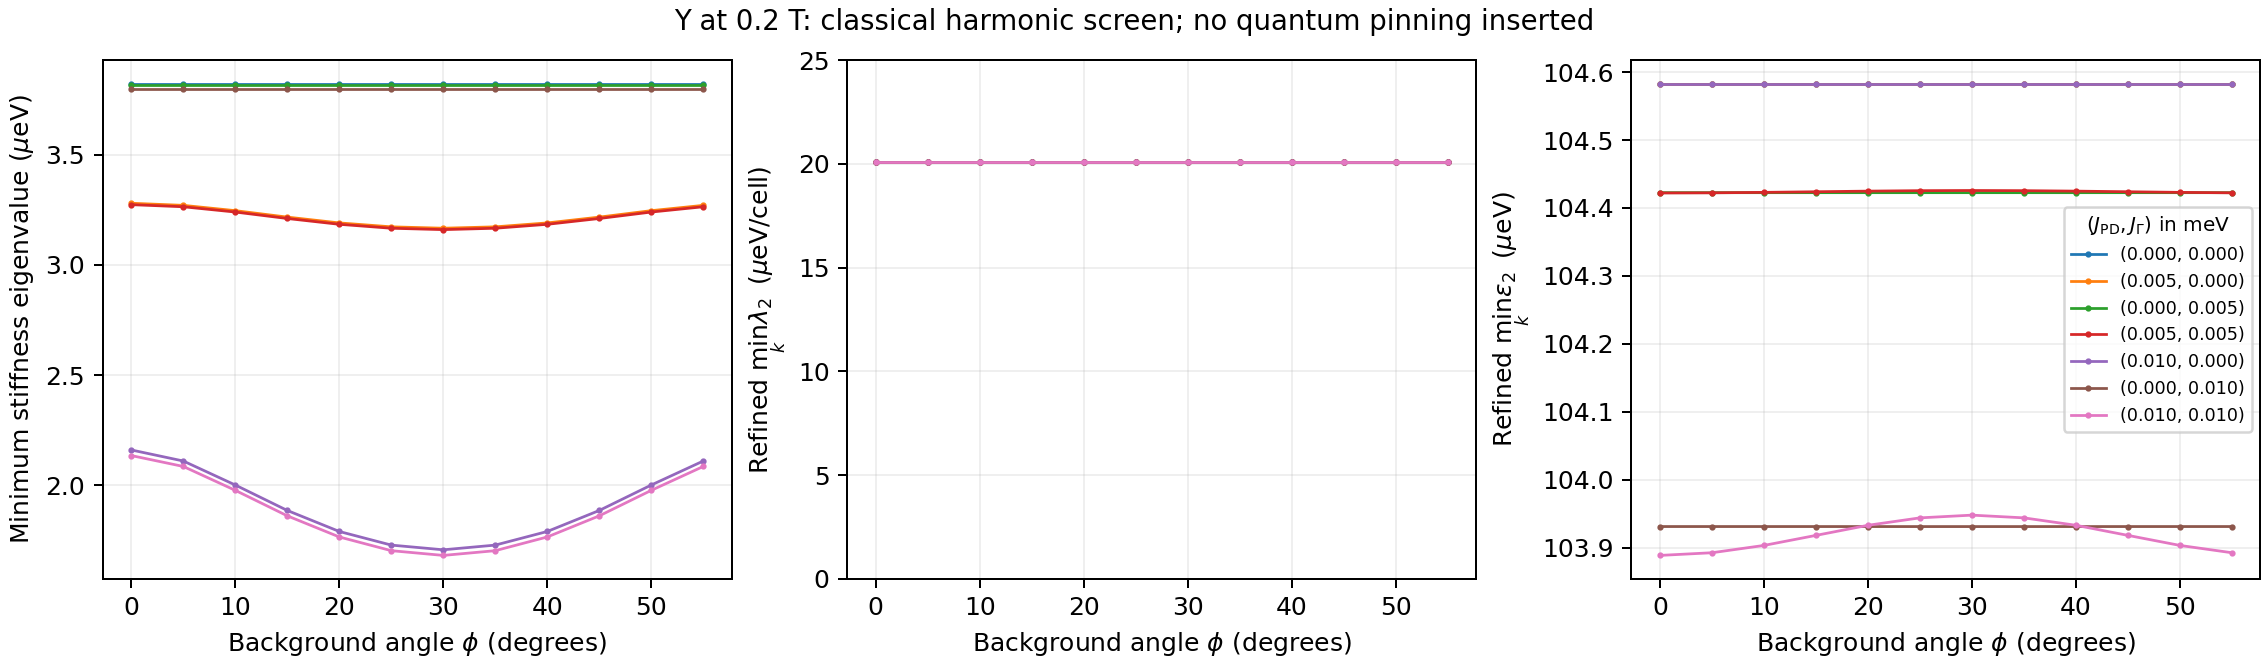
\includegraphics[keepaspectratio]{../../data-space/verification/260917-y-stability/y-stability-screen.png}}

}

\caption{\label{fig-nbcp-y-stability}Full-zone harmonic screen of Y at
0.2 T. Left: the smaller eigenvalue of the relaxed classical stiffness
tensor. Center: the refined second static eigenvalue, whose minimum is
uniform and independent of these SOC pairs within numerical precision.
Right: the refined minimum of the second ordered nonnegative dynamical
energy. Refinement is numerical and does not give certified lower
bounds. No quantum gap or thermal coefficient is included.}

\end{figure}%

The result supports using a single phase as the candidate
long-wavelength coordinate at these parameter points. Finite grids,
finite angular sampling and local minimum searches do not prove
stability for every momentum and parameter. In particular, the test has
not established a thermodynamic phase boundary, a hard-mode correlation
length, the absence of competing density domains, or a
finite-temperature algebraic phase. The angular matching below retains
the observed angle dependence of the gradient tensor and assesses it
together with the higher harmonics of the angular potential.

\subsection{Angular matching of Y stiffness and
potential}\label{sec-nbcp-y-angular-matching}

The angular matching at \(B=0.2\) T separates two approximations:
replacing the classical tensor \(\rho(\phi)\) by a constant, and
retaining only the sixth harmonic of the leading vacuum energy. These
approximations have different accuracies. At \(J_{\rm PD}=0.010\) meV,
freezing the gradient coefficient produces a much larger error than
truncating the potential to its sixth harmonic. The calculation uses the
same seven SOC pairs as the harmonic screen, the fixed classical Y orbit
and the static elimination in Eq.~\ref{eq-nbcp-y-soc-static-schur}. No
quantum relaxation of the five hard coordinates or quantum gradient
correction is included.

\textbf{The tensor over the complete phase circle.} The tensor is
evaluated on successively refined uniform grids of 72, 144, 288 and 576
angles over \(2\pi\). Its Cartesian components contain second and fourth
harmonics. In the chosen spatial axes, their numerical representation is

\begin{equation}\phantomsection\label{eq-nbcp-y-angular-tensor}{
\begin{aligned}
\rho(\phi)&=\bar\rho I_2+
\begin{pmatrix}\operatorname{Re}z(\phi)&\operatorname{Im}z(\phi)\\
\operatorname{Im}z(\phi)&-\operatorname{Re}z(\phi)\end{pmatrix},\\
z(\phi)&=-r_2 e^{2i\phi}+r_4 e^{-4i\phi},\qquad
\langle\rho(\phi)\rangle_\phi=\bar\rho I_2.
\end{aligned}
}\end{equation}

Here \(r_2,r_4\) and \(\bar\rho\) have units of meV and depend on the
couplings and field; \(r_2,r_4\) are nonnegative at the positive SOC
values tested here. This is a representation of the calculated classical
coefficient at this field, not a fit for arbitrary field or a thermal
stiffness. For pure PD at 0.010 meV,
\((\bar\rho,r_2,r_4)=(0.0024436903,0.0005097814,0.0002265658)\) meV. For
pure Gamma at 0.010 meV, these become \((0.0038106162,0.0000127445,0)\)
meV. With both couplings equal to 0.010 meV, they are
\((0.0024309458,0.0005225260,0.0002265658)\) meV.

The second and fourth component harmonics respect tensor covariance. If
\(R\) rotates the spatial axes by \(\pi/3\), then
\(\rho(\phi+\pi/3)=R\rho(\phi)R^{\mathsf T}\). Thus the scalar sixfold
selection rule must not be imposed separately on \(\rho_{xx}\),
\(\rho_{xy}\) and \(\rho_{yy}\). The eigenvalues, determinant and
principal directions follow as

\begin{equation}\phantomsection\label{eq-nbcp-y-angular-invariants}{
\begin{aligned}
\rho_\pm(\phi)&=\bar\rho\pm\sqrt{r_2^2+r_4^2-2r_2r_4\cos6\phi},\\
\det\rho(\phi)&=\bar\rho^2-r_2^2-r_4^2+2r_2r_4\cos6\phi,\\
\vartheta_+(\phi)&=\tfrac12\arg z(\phi)\pmod\pi.
\end{aligned}
}\end{equation}

The last angle is the direction of the larger eigenvalue and is
undefined for an isotropic tensor. On the pure-Gamma axis, both
eigenvalues and the determinant are constant, but their principal axes
rotate with \(\phi\). A constant \(\sqrt{\det\rho}\) therefore does not
imply a constant tensor over the compact phase circle. The
area-preserving coordinate change used below for a fixed tensor cannot
remove this phase-dependent rotation by one global spatial
transformation.

To quantify the constant approximation, choose the angular mean
\(\rho_{\rm c}=\bar\rho I_2\) and compare directional gradient energies
relative to the full tensor:

\begin{equation}\phantomsection\label{eq-nbcp-y-angular-gradient-error}{
\epsilon_\rho=\max_{\phi,\,\widehat{\mathbf q}}
\frac{\left|\widehat{\mathbf q}^{\mathsf T}
[\rho_{\rm c}-\rho(\phi)]\widehat{\mathbf q}\right|}
{\widehat{\mathbf q}^{\mathsf T}\rho(\phi)\widehat{\mathbf q}}.
}\end{equation}

The angular maximum is sampled; the directional maximum at each angle is
obtained from the eigenvalues of
\(\rho^{-1/2}(\rho_{\rm c}-\rho)\rho^{-1/2}\). This specifies an
approximation and its error rather than an optimized or renormalized
matching prescription. Freezing the tensor at \(\phi=0\) instead gives
larger whole-orbit errors: about 59.7\% for pure PD at 0.010 meV and
62.1\% for the equal mixed case.

\begin{longtable}[]{@{}
  >{\raggedleft\arraybackslash}p{(\linewidth - 8\tabcolsep) * \real{0.2000}}
  >{\raggedleft\arraybackslash}p{(\linewidth - 8\tabcolsep) * \real{0.2000}}
  >{\raggedleft\arraybackslash}p{(\linewidth - 8\tabcolsep) * \real{0.2000}}
  >{\raggedright\arraybackslash}p{(\linewidth - 8\tabcolsep) * \real{0.2000}}
  >{\raggedleft\arraybackslash}p{(\linewidth - 8\tabcolsep) * \real{0.2000}}@{}}
\toprule\noalign{}
\begin{minipage}[b]{\linewidth}\raggedleft
\(J_{\rm PD}\) (meV)
\end{minipage} & \begin{minipage}[b]{\linewidth}\raggedleft
\(J_\Gamma\) (meV)
\end{minipage} & \begin{minipage}[b]{\linewidth}\raggedleft
\(\bar\rho\) (meV)
\end{minipage} & \begin{minipage}[b]{\linewidth}\raggedright
Range of \(\sqrt{\det\rho}\) (meV)
\end{minipage} & \begin{minipage}[b]{\linewidth}\raggedleft
\(\epsilon_\rho\)
\end{minipage} \\
\midrule\noalign{}
\endfirsthead
\toprule\noalign{}
\begin{minipage}[b]{\linewidth}\raggedleft
\(J_{\rm PD}\) (meV)
\end{minipage} & \begin{minipage}[b]{\linewidth}\raggedleft
\(J_\Gamma\) (meV)
\end{minipage} & \begin{minipage}[b]{\linewidth}\raggedleft
\(\bar\rho\) (meV)
\end{minipage} & \begin{minipage}[b]{\linewidth}\raggedright
Range of \(\sqrt{\det\rho}\) (meV)
\end{minipage} & \begin{minipage}[b]{\linewidth}\raggedleft
\(\epsilon_\rho\)
\end{minipage} \\
\midrule\noalign{}
\endhead
\bottomrule\noalign{}
\caption{Angular stiffness harmonics and errors from replacing the tensor by its mean.}\label{tab-nbcp-07-y-phase-2}\\
\endlastfoot
0 & 0 & 0.00382336 & 0.00382336 & 0 \\
0.005 & 0 & 0.00347844 & 0.00346446--0.00347279 & 9.84\% \\
0 & 0.005 & 0.00382017 & 0.00382017 & 0.0835\% \\
0.005 & 0.005 & 0.00347526 & 0.00346098--0.00346941 & 9.96\% \\
0.010 & 0 & 0.00244369 & 0.00233011--0.00242722 & 43.13\% \\
0 & 0.010 & 0.00381062 & 0.00381059 & 0.3356\% \\
0.010 & 0.010 & 0.00243095 & 0.00231265--0.00241286 & 44.54\% \\
\end{longtable}

\textbf{The angular potential and curvature.} The classical energy is
constant along this orbit. Its leading angular potential is therefore
the zero-point contribution \(e_{\rm zp}(\phi)\) per physical spin.
Fourier coefficients are extracted over the full circle before
discarding any harmonics:

\begin{equation}\phantomsection\label{eq-nbcp-y-angular-potential}{
\begin{aligned}
v(\phi)&=e_{\rm zp}(\phi)-\langle e_{\rm zp}\rangle_\phi
=\sum_{n\geq1}[a_n\cos(n\phi)+b_n\sin(n\phi)],\\
\lambda_n&=\sqrt{a_n^2+b_n^2},\qquad
v_6(\phi)=a_6\cos6\phi+b_6\sin6\phi,\\
C_\phi=v''(\phi_*)&=-\sum_{n\geq1}n^2
[a_n\cos(n\phi_*)+b_n\sin(n\phi_*)].
\end{aligned}
}\end{equation}

The coefficients and \(C_\phi\) are in meV/spin; the continuum potential
density is \(v/a_{\rm spin}\). The factor \(n^2\) explains why a small
energy harmonic can have a larger effect on local pinning. For a pure
sixth harmonic, the minimum curvature is \(36\lambda_6\). We compare
that value with the curvature of the resolved multi-harmonic potential
at its minimum, and separately define the energy error
\(\epsilon_E=\max_\phi|v-v_6|/\lambda_6\). Neither diagnostic contains a
quantum correction to the spatial stiffness.

The saved current-Hamiltonian scans on the individual SOC axes are
reused at \(N=12,24,48\) and 72 angles. At \(N=48\), adding the
interleaved angles gives 144 samples. Full-circle mixed-SOC scans are
computed separately at \(N=24,48\); they are not obtained by adding the
two pure-axis energies. All six nonzero cases are checked at \(N=96\)
with 72 angles. Each momentum quadrature uses the reciprocal-cell
midpoint grid and six rotated copies, avoiding the defective
zero-frequency point without an onsite shift. This preserves the lattice
symmetry of the quadrature; the Fourier extraction itself imposes no
sixfold selection rule. Spectral covariance is also checked at fresh,
unaveraged momenta.

The finest momentum-grid estimates are:

\begin{longtable}[]{@{}
  >{\raggedleft\arraybackslash}p{(\linewidth - 8\tabcolsep) * \real{0.2000}}
  >{\raggedleft\arraybackslash}p{(\linewidth - 8\tabcolsep) * \real{0.2000}}
  >{\raggedleft\arraybackslash}p{(\linewidth - 8\tabcolsep) * \real{0.2000}}
  >{\raggedleft\arraybackslash}p{(\linewidth - 8\tabcolsep) * \real{0.2000}}
  >{\raggedleft\arraybackslash}p{(\linewidth - 8\tabcolsep) * \real{0.2000}}@{}}
\toprule\noalign{}
\begin{minipage}[b]{\linewidth}\raggedleft
\(J_{\rm PD}\) (meV)
\end{minipage} & \begin{minipage}[b]{\linewidth}\raggedleft
\(J_\Gamma\) (meV)
\end{minipage} & \begin{minipage}[b]{\linewidth}\raggedleft
\(\lambda_6\) (meV/spin)
\end{minipage} & \begin{minipage}[b]{\linewidth}\raggedleft
\(\lambda_{12}/\lambda_6\)
\end{minipage} & \begin{minipage}[b]{\linewidth}\raggedleft
Sixth-only curvature error
\end{minipage} \\
\midrule\noalign{}
\endfirsthead
\toprule\noalign{}
\begin{minipage}[b]{\linewidth}\raggedleft
\(J_{\rm PD}\) (meV)
\end{minipage} & \begin{minipage}[b]{\linewidth}\raggedleft
\(J_\Gamma\) (meV)
\end{minipage} & \begin{minipage}[b]{\linewidth}\raggedleft
\(\lambda_6\) (meV/spin)
\end{minipage} & \begin{minipage}[b]{\linewidth}\raggedleft
\(\lambda_{12}/\lambda_6\)
\end{minipage} & \begin{minipage}[b]{\linewidth}\raggedleft
Sixth-only curvature error
\end{minipage} \\
\midrule\noalign{}
\endhead
\bottomrule\noalign{}
\caption{Leading angular-potential harmonics at the finest sampled momentum mesh.}\label{tab-nbcp-07-y-phase-3}\\
\endlastfoot
0.005 & 0 & \(1.187\times10^{-7}\) & \(2.120\times10^{-4}\) &
0.0847\% \\
0 & 0.005 & \(2.5\times10^{-14}\) & unresolved & unresolved \\
0.005 & 0.005 & \(1.259\times10^{-7}\) & \(2.111\times10^{-4}\) &
0.0844\% \\
0.010 & 0 & \(1.437\times10^{-6}\) & \(2.885\times10^{-3}\) & 1.142\% \\
0 & 0.010 & \(1.643\times10^{-12}\) & unresolved & unresolved \\
0.010 & 0.010 & \(1.670\times10^{-6}\) & \(2.885\times10^{-3}\) &
1.143\% \\
\end{longtable}

For the pure-PD and mixed cases at 0.010 meV, \(\epsilon_E\) is about
0.289\%, while the sum of resolved higher-harmonic amplitudes weighted
by \(n^2\), divided by \(36\lambda_6\), is about 1.16\%. Their
eighteenth-harmonic amplitude ratios are \(9.54\times10^{-7}\) and
\(2.46\times10^{-6}\), respectively. The twelfth harmonic therefore
dominates the correction to the minimum curvature at these points. The
zero-SOC control retains its exact continuous symmetry and has no
physical angular pinning.

These coefficients are leading order in \(1/S\). At \(S=1/2\) and
\(J_{\rm PD}=0.010\) meV, the order-\(S^0\) angular curvature of Y is
\(-27\) times the zero-point curvature
(Appendix Section~\ref{sec-nbcp-gap-validity}). Neither the size of
\(\lambda_6\) nor its sign, which decides which of the two sixfold
orientations is selected, is fixed by the expansion. The symmetry
statements, a sixfold potential at \(J_\Gamma=0\) and the order of each
harmonic in the couplings, do not depend on it.

Mixed SOC changes the sixth coefficient appreciably even though the
pure-Gamma potential is tiny. Adding the pure-PD and pure-Gamma sixth
coefficients underestimates the directly computed mixed coefficient by
5.71\% at \((0.005,0.005)\) meV and 13.96\% at \((0.010,0.010)\) meV,
relative to the mixed result. The coexistence of the two interactions
changes the vacuum spectrum; the small pure-Gamma energy alone does not
control this cross effect. The spin-rotation selection rule of
Section~\ref{sec-nbcp-yv-selection-rule} allows a
\(J_{\rm PD}^2J_\Gamma^2\) contribution of this kind.

\begin{figure}[htbp]

\centering{

\nbcpbounded{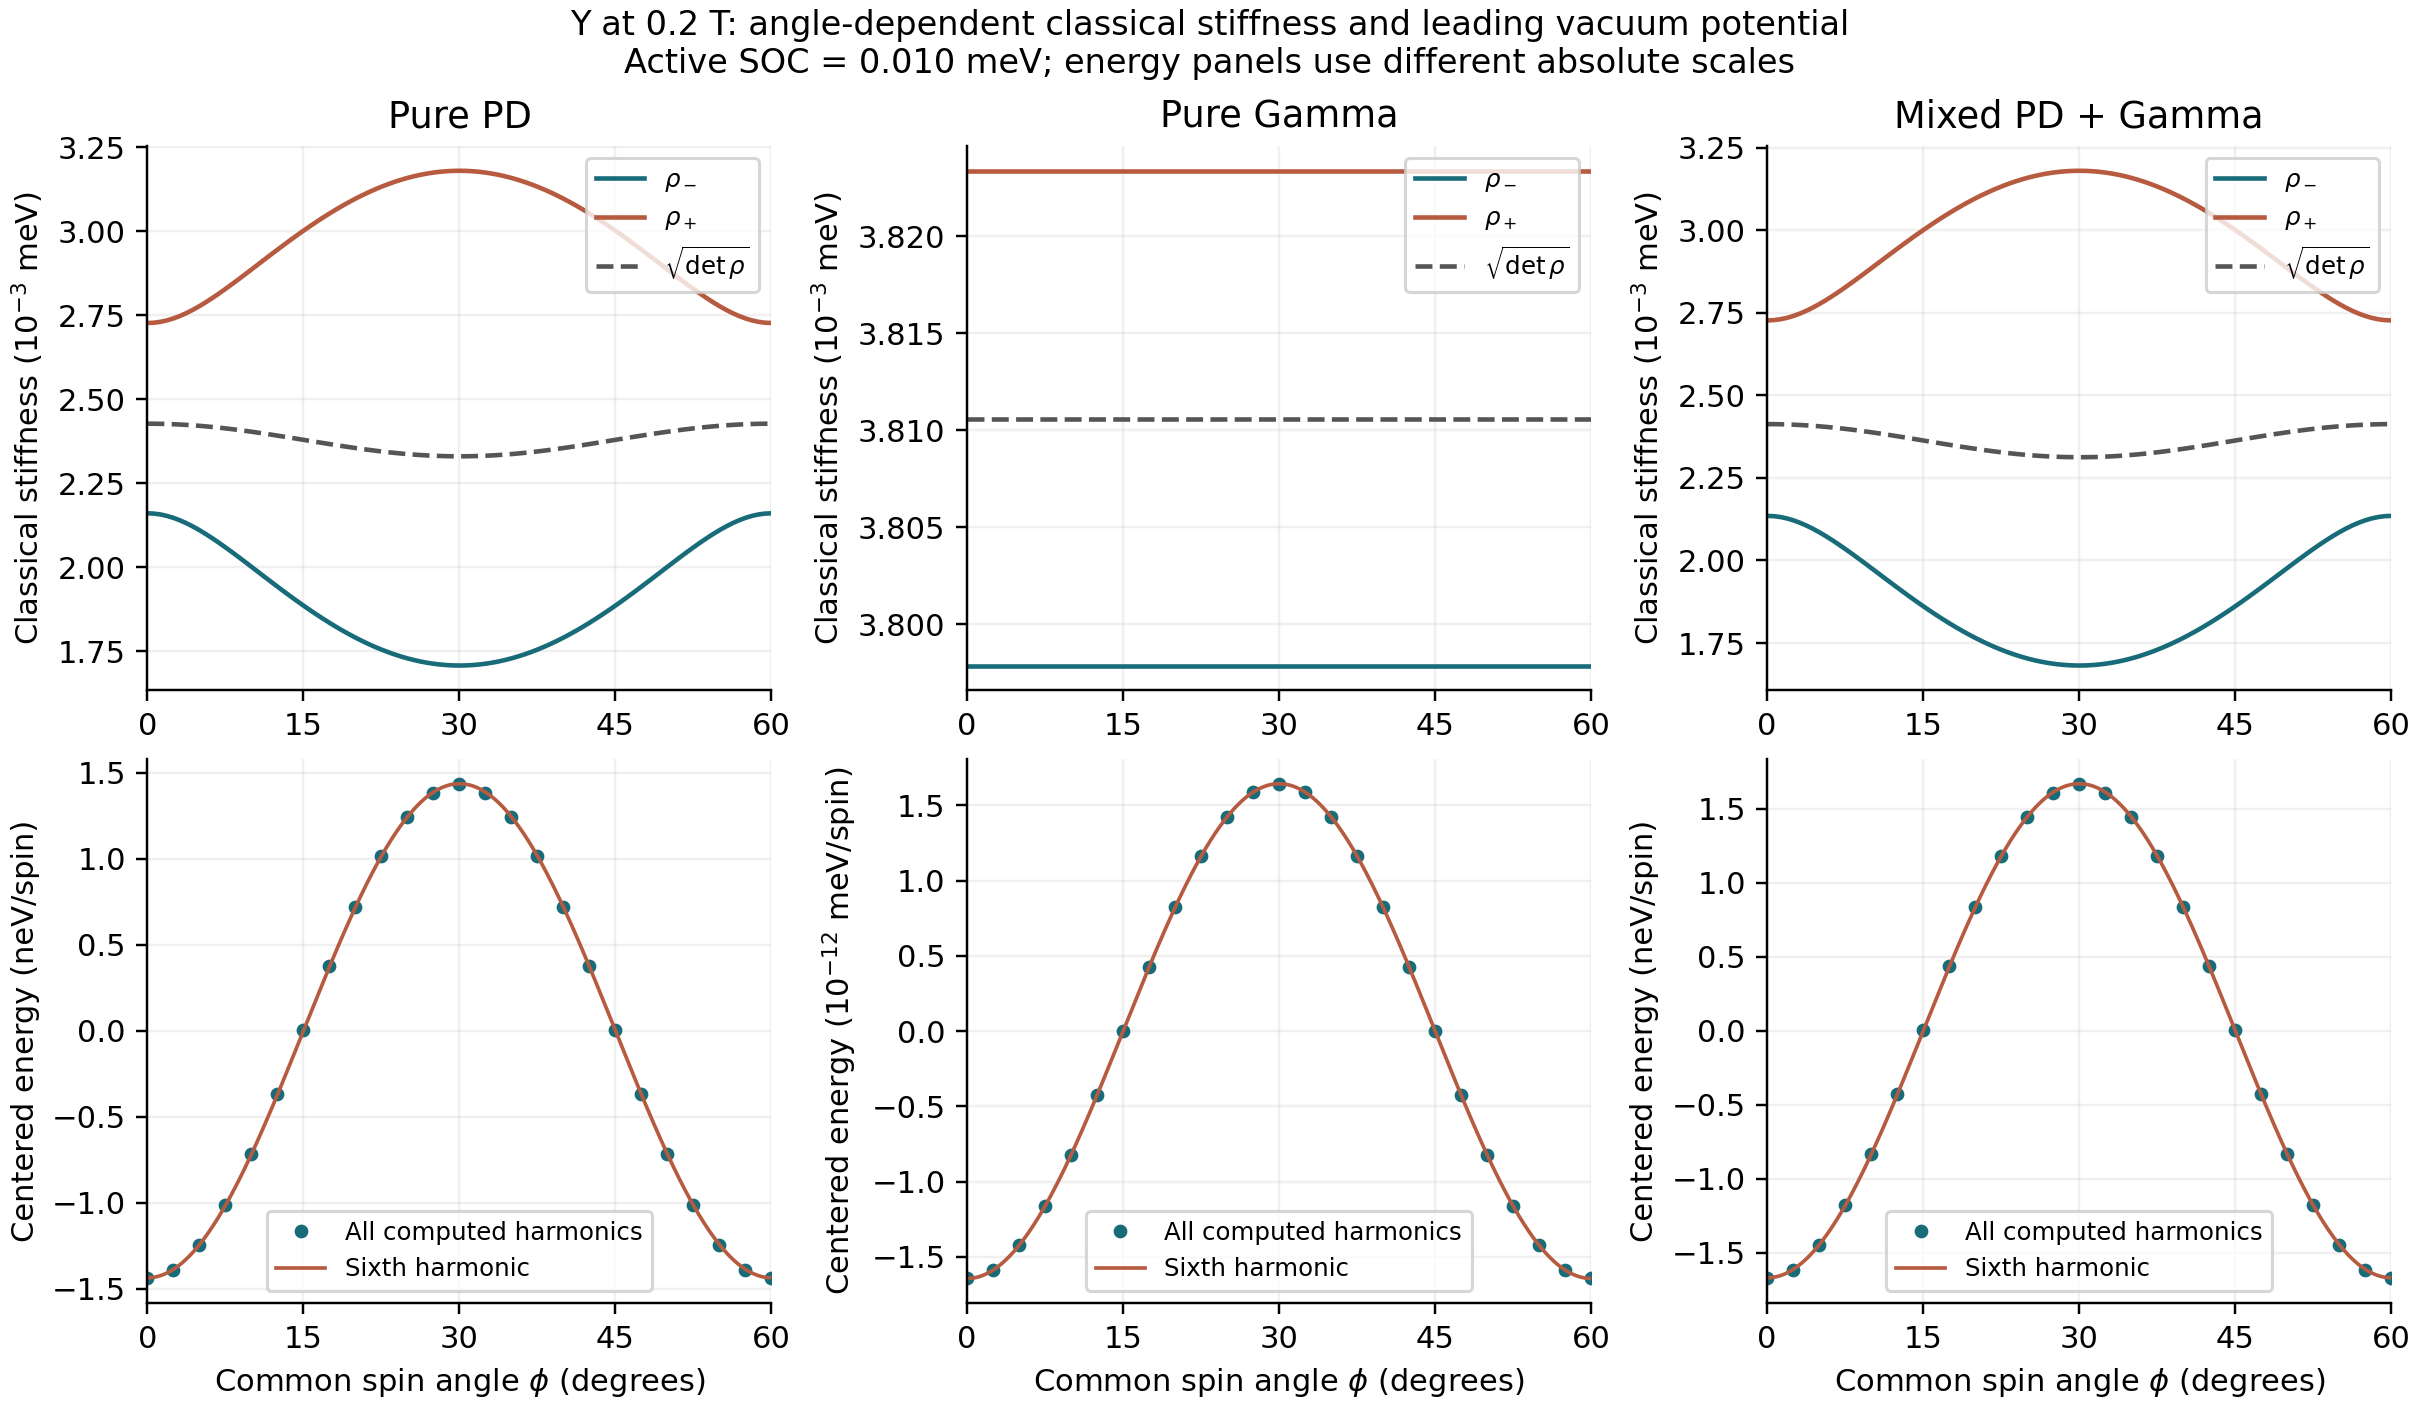
\includegraphics[keepaspectratio]{../../data-space/verification/260918-y-angular-matching/y-angular-matching.png}}

}

\caption{\label{fig-nbcp-y-angular-matching}Y angular matching at 0.2 T
for pure PD, pure Gamma and equal mixed SOC, with each active
coefficient equal to 0.010 meV. Top: the two classical stiffness
eigenvalues and the square root of the determinant. Bottom: centered
vacuum energies from the 144-angle N48 scans and their sixth harmonics.
The pure-Gamma energy panel uses a much smaller absolute scale. Constant
eigenvalues on that axis coexist with rotating principal directions.
These are classical gradient and leading quantum potential coefficients,
not thermal matching data.}

\end{figure}%

\textbf{Resolution and interpretation.} Increasing the tensor angular
resolution from 72 to 576 changes the sampled extrema and low-order
Fourier coefficients by less than \(9\times10^{-19}\) meV. The tensor
covariance residual is below \(5\times10^{-18}\) meV; component
amplitudes above fourth order are below \(2\times10^{-19}\) meV. At
fresh background angles and \(ka=0.001\), the finite-momentum static and
production paired-dispersion estimates differ from the derivative-based
coefficient by at most \(5.6\times10^{-7}\) and \(4.7\times10^{-7}\)
relatively. These are convergence checks within the same classical
model.

For the potential, doubling the angular resolution changes the
amplitudes below harmonic 36 by at most \(1.5\times10^{-18}\) meV/spin
at fixed \(N=48\). The sixth coefficients in the PD-containing cases
change by \(2.1\times10^{-5}\)--\(3.7\times10^{-5}\) relatively from
\(N=48\) to 96. These observed differences are convergence diagnostics,
not certified quadrature error bounds. The independent
Cartesian-to-Nambu matrix comparison differs from the production
Hamiltonian by less than \(5.6\times10^{-17}\) meV, and direct dynamical
eigenvalue sums reproduce the vacuum energy within \(1.3\times10^{-17}\)
meV/spin.

Pure-Gamma requires a separate resolution statement. An empirical
coefficient floor, the larger of
\(100\epsilon_{\rm mach}\max|e_{\rm zp}|\) and the largest non-sixfold
amplitude, is approximately \(1.8\times10^{-16}\) meV/spin. It is a
conservative numerical diagnostic, not an uncertainty distribution or
rigorous error bound. The sixth coefficient lies above it, but the
higher coefficients do not. At \(J_\Gamma=0.005\) and 0.010 meV, this
floor is respectively about 0.7\% and 0.011\% of \(\lambda_6\). The
smaller observed mesh changes do not justify extra physical precision.
Setting unresolved coefficients to zero would make the sixth-only
curvature error vanish by construction; the table therefore reports it
as unresolved. Weighting a floor-sized uncertainty at every unresolved
sampled harmonic by \(n^2\) gives a curvature diagnostic of roughly
\(2.7\times10^{-12}\) meV/spin at 72 angles. This exceeds the
small-Gamma sixth-harmonic curvature and is about 4.6\% of the
larger-Gamma value. It is deliberately conservative and does not bound
the unmeasured harmonics beyond the angular Nyquist limit.

A separate five-point energy derivative at \(N=96\) corroborates the
resolved Fourier curvature: for the four PD-containing cases, its
relative discrepancy decreases to less than \(2.8\times10^{-6}\) at a
step of 0.02 rad. For pure Gamma at 0.005 meV, reducing the step instead
increases the discrepancy from about 0.25\% to 1.9\%, directly exposing
cancellation noise. At 0.010 meV, steps of 0.04 and 0.02 rad give
differences near \(3\times10^{-5}\). These comparisons support the
leading signal without resolving the tiny higher harmonics. The full
dynamical spectra at 37 fresh unaveraged momenta satisfy the combined
\(60^\circ\) rotation to within \(10^{-15}\) meV, and 49 off-grid tensor
evaluations reproduce Eq.~\ref{eq-nbcp-y-angular-tensor} within
\(4\times10^{-18}\) meV.

The practical result is that a sixth-harmonic potential is accurate at
the percent level in local curvature for the tested PD-containing
points, whereas their constant-gradient approximation can be much less
accurate. Subsequent defect calculations should retain the angular
tensor and at least the sixth and twelfth potential harmonics when using
these microscopic inputs. On the pure-Gamma axis, a constant tensor is a
much closer approximation, while the extremely weak potential demands
its own numerical error assessment. This remains a mixture of classical
stiffness and leading zero-point potential at \(T=0\). Quantum gradient
corrections, finite-temperature matching, vortex-core weights and a
thermal RG trajectory are not supplied by this calculation.

\subsection{Nonlinear smooth-wave test of the Y gradient
theory}\label{sec-nbcp-y-nonlinear-gradient}

The angular matching can be tested beyond infinitesimal spin deviations
without first simulating a thermal transition. At \(B=0.2\) T, consider
the three pairs \((J_{\rm PD},J_\Gamma)=(0.005,0)\), \((0.010,0)\) and
\((0.010,0.010)\) meV. On a periodic array of \(L\times L\) magnetic
cells, prescribe the phase of the transverse staggered component and
relax the other five coordinates in every cell:

\begin{equation}\phantomsection\label{eq-nbcp-y-nonlinear-phase}{
\arg(n^+_{A,\mathbf R}-n^+_{B,\mathbf R})
=\phi_{\mathbf R}=\phi_0+A\cos(\mathbf q\cdot\mathbf R),
\qquad n_i^+=n_i^x+\mathrm i n_i^y.
}\end{equation}

Here \(\mathbf n_i\) are unit spins. Each spin is parameterized as
\(\mathbf n_i=\mathbf n_i^{(0)}\sqrt{1-x_i^2-y_i^2}+\mathbf e_{1i}x_i+\mathbf e_{2i}y_i\),
with the background and tangent frame rotated by the prescribed cell
phase. The five-coordinate chart imposes \(y_A=y_B\); it preserves the
staggered phase exactly while allowing independent polar deviations and
the remaining transverse motions. The calculation minimizes the full
classical exchange and field energy, rather than its quadratic
expansion. Coordinate bounds keep the positive-root chart regular, but
none is active in the final configurations. This is a search for
constrained local minima within the Y branch, not for competing density
domains or global minima.

The comparison uses \(\phi_0=0,\pi/6\), amplitudes \(A=0.02,0.2,0.5,1\)
rad and \(L=8,16,32,64\), with an additional \(L=128\) refinement at
\(A=0.02,1\). Reciprocal-cell modes \((1,1)\) and \((1,-1)\) give waves
along the numerical Cartesian axes, with wavelengths \(3La/2\) and
\(\sqrt{3}La/2\), respectively. There are 216 cases; the largest
contains 49,152 spins. No zero-point pinning potential or thermal
correction is added.

The continuum energy per spin predicted by the previously matched tensor
is

\begin{equation}\phantomsection\label{eq-nbcp-y-nonlinear-energy}{
\Delta e_{\rm cont}=\frac{a_{\rm spin}A^2}{2}
\int_0^{2\pi}\frac{dt}{2\pi}\sin^2t\,
\mathbf q^{\mathsf T}\rho(\phi_0+A\cos t)\mathbf q,
\qquad a_{\rm spin}=\frac{\sqrt{3}a^2}{2}.
}\end{equation}

Keeping \(\rho(\phi_0)\) fixed instead gives a separate diagnostic of
the error caused by discarding its angular dependence. The table reports
the largest absolute relative energy error over the three SOC pairs, two
directions and two background angles, with the relaxed lattice energy as
denominator.

All four amplitudes have errors below 1\% at \(L=64\), where the
wavelengths are approximately \(55a\) and \(96a\). At \(A=1\), the error
falls further to 0.24\% at \(L=128\), while the frozen-tensor error
remains about 10\%. The relaxed internal deviations also decrease with
wavelength. These observations support the leading, angle-dependent
classical gradient energy for the sampled smooth configurations,
including finite phase excursions. The 1\% observation is not a
universal wavelength cutoff.

\begin{longtable}[]{@{}
  >{\raggedleft\arraybackslash}p{(\linewidth - 6\tabcolsep) * \real{0.2500}}
  >{\raggedleft\arraybackslash}p{(\linewidth - 6\tabcolsep) * \real{0.2500}}
  >{\raggedleft\arraybackslash}p{(\linewidth - 6\tabcolsep) * \real{0.2500}}
  >{\raggedleft\arraybackslash}p{(\linewidth - 6\tabcolsep) * \real{0.2500}}@{}}
\toprule\noalign{}
\begin{minipage}[b]{\linewidth}\raggedleft
\(L\)
\end{minipage} & \begin{minipage}[b]{\linewidth}\raggedleft
Full \(\rho(\phi)\), \(A=0.02\)
\end{minipage} & \begin{minipage}[b]{\linewidth}\raggedleft
Full \(\rho(\phi)\), \(A=1\)
\end{minipage} & \begin{minipage}[b]{\linewidth}\raggedleft
Frozen \(\rho(\phi_0)\), \(A=1\)
\end{minipage} \\
\midrule\noalign{}
\endfirsthead
\toprule\noalign{}
\begin{minipage}[b]{\linewidth}\raggedleft
\(L\)
\end{minipage} & \begin{minipage}[b]{\linewidth}\raggedleft
Full \(\rho(\phi)\), \(A=0.02\)
\end{minipage} & \begin{minipage}[b]{\linewidth}\raggedleft
Full \(\rho(\phi)\), \(A=1\)
\end{minipage} & \begin{minipage}[b]{\linewidth}\raggedleft
Frozen \(\rho(\phi_0)\), \(A=1\)
\end{minipage} \\
\midrule\noalign{}
\endhead
\bottomrule\noalign{}
\caption{Finite-wavelength errors of the nonlinear Y gradient description.}\label{tab-nbcp-07-y-phase-4}\\
\endlastfoot
8 & 16.05\% & 14.45\% & 20.80\% \\
16 & 6.89\% & 7.28\% & 14.55\% \\
32 & 2.06\% & 3.04\% & 11.38\% \\
64 & 0.54\% & 0.90\% & 10.34\% \\
128 & 0.14\% & 0.24\% & 10.06\% \\
\end{longtable}

\begin{figure}[htbp]

\centering{

\nbcpbounded{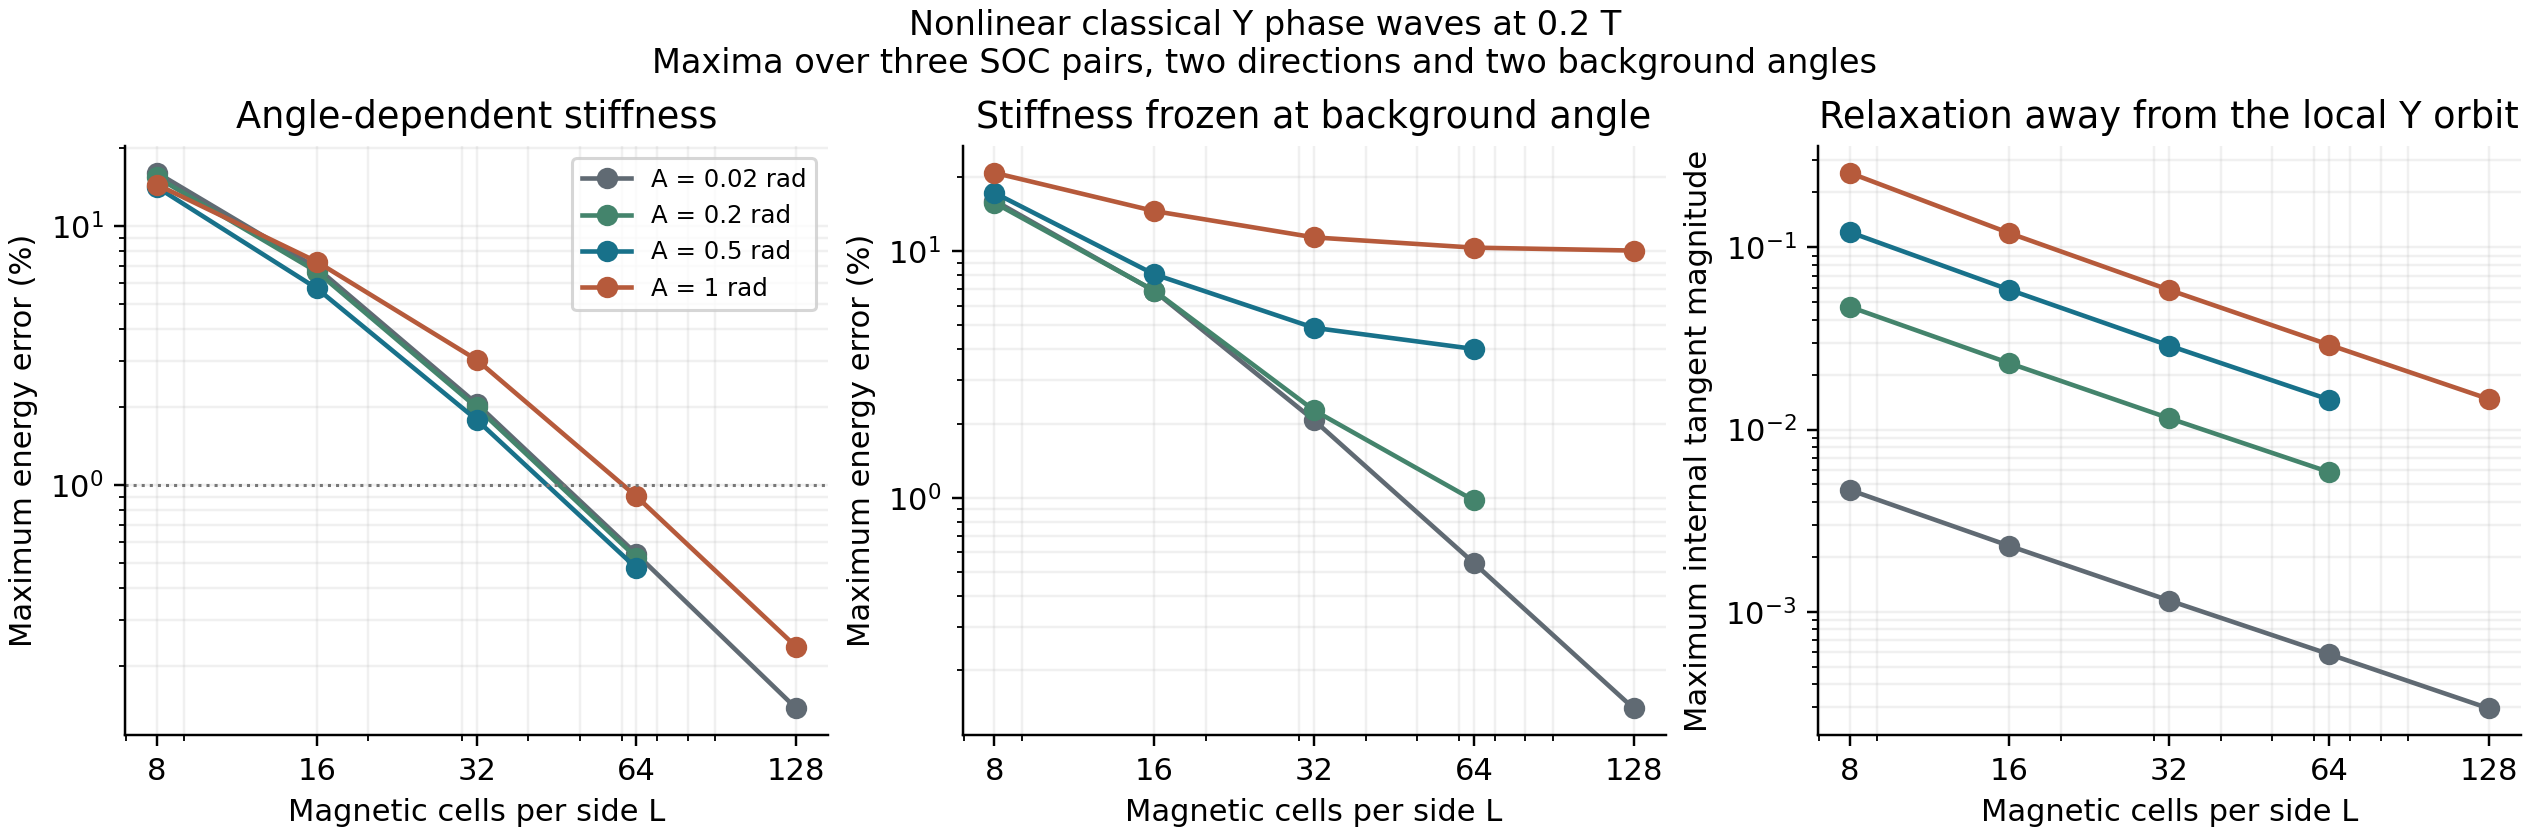
\includegraphics[keepaspectratio]{../../data-space/verification/260918-y-nonlinear-gradient/nonlinear-gradient-convergence.png}}

}

\caption{\label{fig-nbcp-y-nonlinear-gradient}Nonlinear classical
smooth-wave comparison at 0.2 T. Each curve shows a maximum over the
tested SOC pairs, directions and background angles. Left: energy error
with the full angular tensor. Center: error with the tensor frozen at
the background angle. Right: the largest relaxed tangent displacement
from the local Y orbit. Increasing L increases the wavelength; it is not
a thermal finite-size scaling study. Only the smallest and largest
amplitudes were continued to L=128.}

\end{figure}%

\textbf{Constraint matching and numerical checks.} A phase attached to a
magnetic cell differs at finite momentum from the physical-site Fourier
convention used in the earlier kernel. The harmonic comparison therefore
transforms that kernel with \(K_{\rm cell}=UKU^\dagger\), where \(U\)
contains \(e^{\mathrm i\mathbf q\cdot\mathbf r_i}\) on both tangent
blocks, before eliminating the same five constrained coordinates. At
\(A=5\times10^{-4}\) rad, the full lattice energy agrees with this
finite-momentum harmonic prediction to within \(5.9\times10^{-7}\)
relatively. Thus the continuum discrepancy contains finite-gradient and
cell-coordinate corrections as well as finite-amplitude effects; it
should not all be labeled a nonlinear interaction correction.

An explicit bond enumeration agrees with the vectorized energy within
\(5.3\times10^{-17}\) meV, and a directional finite-difference check of
the analytic gradient has a discrepancy below \(5.6\times10^{-11}\)
under the diagnostic's normalization. Across the main scan, the largest
residual gradient is \(1.9\times10^{-9}\) meV, and spin-length and
phase-constraint residuals are below \(3\times10^{-16}\). Two random
all-cell perturbations at \(L=32\), \(A=1\), \(\phi_0=\pi/6\) in the
second direction return the same energy within \(10^{-18}\) meV/spin for
each SOC pair. Doubling the torus at fixed wavelength in a separate
\(A=0.5\) check changes the relaxed energy by less than
\(1.6\times10^{-18}\) meV/spin. These are local convergence checks, not
proofs of a global minimum.

The scan and numerical checks took 40.6 s with a peak process RSS of 165
MiB on the tested Apple M1 machine with 8 GB memory, before figure and
document generation. Nonlinear classical relaxation at these sizes is
therefore feasible on this computer. The present evidence concerns only
the smooth gradient sector of a local Y description. This smooth-wave
test supplies no density-wall or vortex-core energies, statistical
weights, quantum gradient corrections or temperature-dependent matching.
In particular, the convergence at long wavelengths does not establish a
continuum description for a defect whose core spans only a few lattice
spacings, nor does it validate the clock RG trajectory of the quantum
magnet.

\subsection{Classical walls between Y density
domains}\label{sec-nbcp-y-density-wall}

A density wall changes which sublattice carries the downward spin of the
Y state. It therefore leaves the local chart of a single density domain
used in the smooth-wave test. At \(B=0.2\) T, the full classical spin
energy is minimized on a periodic array of \(L\times W\) magnetic cells.
Two adjacent layers near cell coordinate zero are fixed to the reference
Y state; two layers halfway around the torus are fixed to its cyclic
sublattice permutation followed by a common spin rotation through
\(\Delta\phi\). Every other spin can move on the full unit sphere. These
boundary data create two interfaces without open surfaces. The reported
energy per interface length is

\begin{equation}\phantomsection\label{eq-nbcp-y-density-wall-energy}{
\bar\sigma_{L,W}(\Delta\phi)
=\frac{E_{\rm constrained}-E_{\rm uniform}}{2\ell_\parallel},
\qquad \ell_\parallel=\sqrt{3}Wa,
\qquad d_{\rm walls}=\frac{3La}{4}.
}\end{equation}

The two interfaces need not have identical microscopic cores, so
\(\bar\sigma\) is their average. The fixed slabs also impose phase
twists at finite separation. Thus it is a finite-system excess energy,
not an isolated-wall free energy. No quantum angular potential is added.
The translated uniform domains have equal energies and vanishing torques
to numerical precision in this construction.

The initial scan uses \(L=32,64,128\), \(W=1\) and eight equally spaced
offsets over \(2\pi\) for each of four SOC pairs. For the lowest sampled
branch at \(L=128\), additional calculations vary the initial wall width
and random spin perturbations, increase \(W\) to 4, 8 and 16, and
increase \(L\) to 256 and 512. The other translated domain and the
second magnetic-lattice strip orientation are also sampled. Broad
phase-twist starts test metastability at the opposite pinned offset;
starts containing the third density domain test a possible splitting of
the interface. Altogether 164 relaxed configurations are saved, in
addition to auxiliary reference solves.

\begin{longtable}[]{@{}
  >{\raggedright\arraybackslash}p{(\linewidth - 6\tabcolsep) * \real{0.2000}}
  >{\raggedleft\arraybackslash}p{(\linewidth - 6\tabcolsep) * \real{0.2667}}
  >{\raggedleft\arraybackslash}p{(\linewidth - 6\tabcolsep) * \real{0.2667}}
  >{\raggedleft\arraybackslash}p{(\linewidth - 6\tabcolsep) * \real{0.2667}}@{}}
\toprule\noalign{}
\begin{minipage}[b]{\linewidth}\raggedright
\((J_{\rm PD},J_\Gamma)\) (meV)
\end{minipage} & \begin{minipage}[b]{\linewidth}\raggedleft
\(\bar\sigma_{512,1}\) (meV/\(a\))
\end{minipage} & \begin{minipage}[b]{\linewidth}\raggedleft
Change from \(L=256\)
\end{minipage} & \begin{minipage}[b]{\linewidth}\raggedleft
Density width (\(a\))
\end{minipage} \\
\midrule\noalign{}
\endfirsthead
\toprule\noalign{}
\begin{minipage}[b]{\linewidth}\raggedright
\((J_{\rm PD},J_\Gamma)\) (meV)
\end{minipage} & \begin{minipage}[b]{\linewidth}\raggedleft
\(\bar\sigma_{512,1}\) (meV/\(a\))
\end{minipage} & \begin{minipage}[b]{\linewidth}\raggedleft
Change from \(L=256\)
\end{minipage} & \begin{minipage}[b]{\linewidth}\raggedleft
Density width (\(a\))
\end{minipage} \\
\midrule\noalign{}
\endhead
\bottomrule\noalign{}
\caption{Classical density-wall tensions and widths for the sampled SOC parameters.}\label{tab-nbcp-07-y-phase-5}\\
\endlastfoot
\((0,0)\) & 0.017505 & 0.066\% & 3.09 \\
\((0.005,0)\) & 0.015691 & 0.081\% & 3.46 \\
\((0.010,0)\) & 0.013461 & 0.066\% & 3.80 \\
\((0.010,0.010)\) & 0.011646 & 0.198\% & 3.32 \\
\end{longtable}

These are the lower tested branches at the largest separation, not
certified global minima or extrapolated tensions. The last-size changes
are convergence diagnostics rather than error bounds. To specify the
width without assuming a continuum wall shape, define
\(\mathbf m_l=W^{-1}\sum_w(n^z_{l,w,A},n^z_{l,w,B},n^z_{l,w,C})\) and
\(s_l=|\mathbf m_{l+1}-\mathbf m_l|\). The table uses the participation
width \(w_\rho=(3a/2)(\sum_l s_l)^2/(2\sum_l s_l^2)\), with the factor
two accounting for the two principal interfaces. It measures the spread
of the density change, not a fitted correlation length.

\begin{figure}[htbp]

\centering{

\nbcpbounded{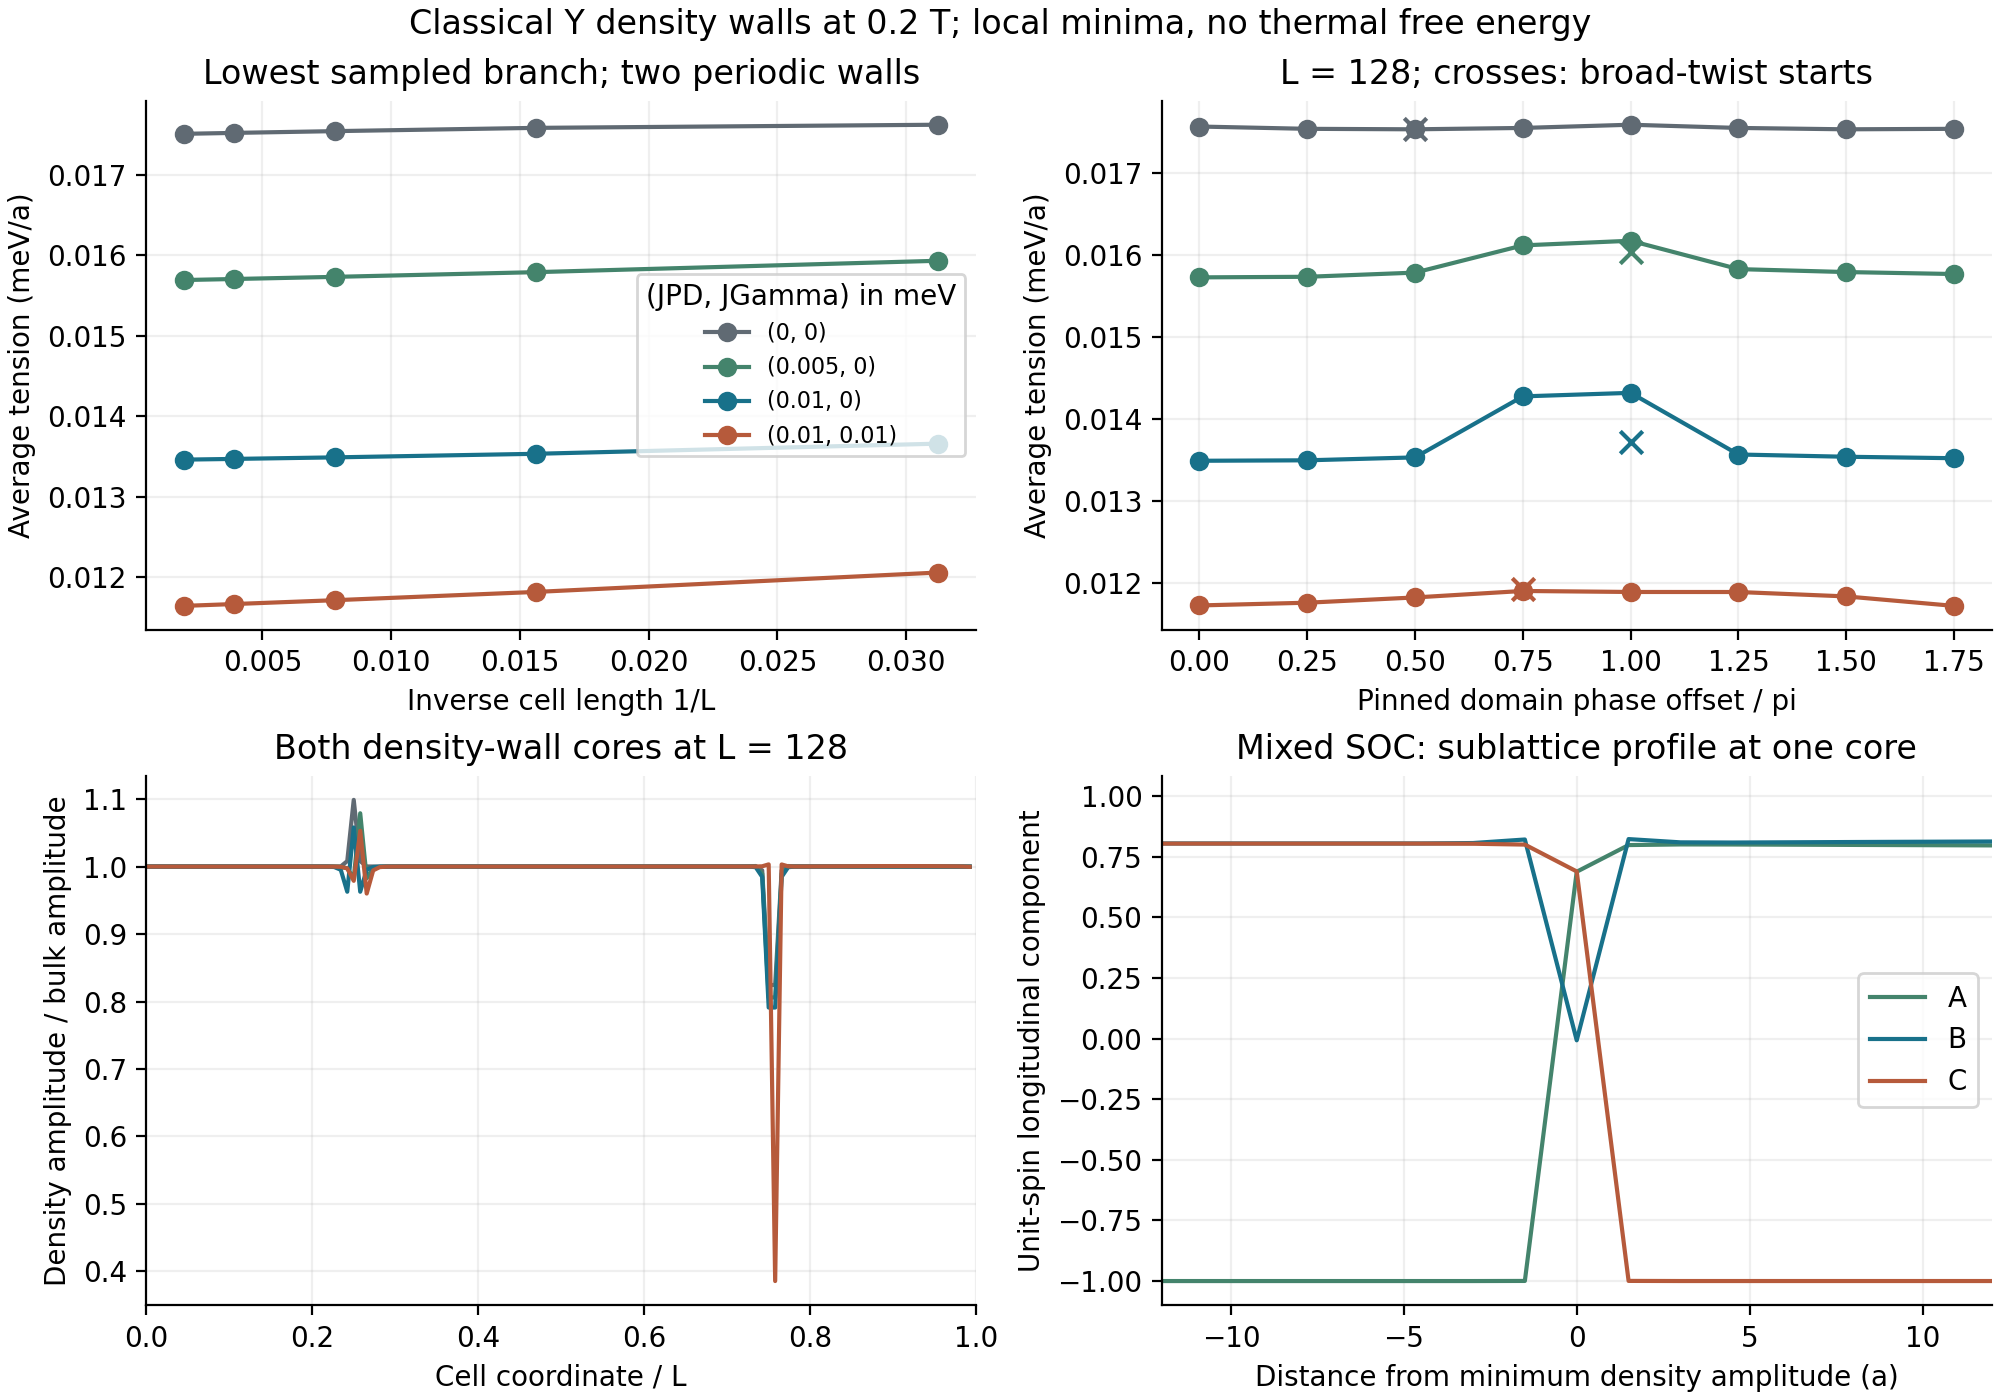
\includegraphics[keepaspectratio]{../../data-space/verification/260918-y-density-wall/density-wall-diagnostic.png}}

}

\caption{\label{fig-nbcp-y-density-wall}Classical Y density-wall
diagnostics at 0.2 T. Top left: lowest sampled excess energy at each
size, with increasing wall separation toward the left. Top right: the
direct eight-offset scan at L=128; crosses show additional starts with a
broad phase twist. Bottom left: the magnitude of the three-sublattice
longitudinal density order in each magnetic cell, normalized by its bulk
value, showing both interfaces. Bottom right: the mixed-SOC sublattice
profile near the core with the strongest density suppression. The two
microscopic cores can differ. All results are constrained classical
local minima.}

\end{figure}%

For the selected \(L=128\) branches, increasing the transverse period
from one to sixteen magnetic cells after random all-spin perturbations
changes the tension by less than \(2\times10^{-13}\) meV/\(a\). The
residual variation along the wall is below \(1.2\times10^{-6}\) in
unit-spin components. This supports local stability of these straight
walls against the sampled transverse perturbations; it does not exclude
another modulated wall. Multiple direct starts agree closely on the
lower branch but also reveal nearby higher minima. A third density
domain in the initial cores remains as a more costly multi-interface
configuration, with roughly twice the excess energy of the lower
two-interface branch. Its energy divided by two interface lengths is not
an elementary-wall tension.

The imposed phase difference requires particular care. For pure PD at
0.010 meV and \(L=512\), direct interpolation at \(\Delta\phi=\pi\)
gives approximately 0.014254 meV/\(a\), while placing the phase offset
in a broad twist before relaxation lowers it to 0.013516 meV/\(a\). The
lower \(\Delta\phi=0\) branch is 0.013461 meV/\(a\). Therefore the
direct phase-offset curve includes metastability and finite-length twist
costs. It does not determine a unique intrinsic phase jump or a
fractional vortex charge bound to a wall; the periodic strips and
networks below do.

\textbf{Forward and backward walls.} The two interfaces of this
construction are not equivalent. Label the domains by \(d=0,1,2\), the
number of cyclic sublattice permutations of the reference Y state. With
the strip axis fixed, one interface takes \(d\) to \(d+1\) when crossed
along the axis and the other takes \(d\) to \(d-1\); call them forward
and backward. A periodic strip without fixed slabs that contains three
walls of one kind, in the order \(0,1,2\) or \(0,2,1\), has three walls
related by translation, so its excess energy divided by three wall
lengths is the tension of that wall. Both strip axes give the same
values. At \(J_{PD}=0\), \(\sigma_{\rm f}=0.01420\) and
\(\sigma_{\rm b}=0.02081\) meV/\(a\); at \(J_{PD}=0.010\) meV,
\(\sigma_{\rm f}=0.011005\) and \(\sigma_{\rm b}=0.015900\) meV/\(a\).
Their means, 0.01750 and 0.01345 meV/\(a\), reproduce the corresponding
rows of Table~\ref{tab-nbcp-07-y-phase-5}, which therefore lists the
average of two different walls rather than an elementary tension.
Because \(\sigma_{\rm b}<2\sigma_{\rm f}\), a backward wall does not
split into two forward walls enclosing a strip of the third domain.

\textbf{Phase at the walls.} At \(J_{PD}=0\) the absolute angle is free,
but a forward wall prefers a large phase jump. With the two slabs of the
construction above held at equal angles, the jump across the forward
wall, extrapolated to its centre from both sides, has magnitude 2.44,
2.79 and 2.96 at \(L=128\), 256 and 512. It approaches \(\pi\) as the
twist imposed by the slabs spreads over a longer domain. Three forward
walls in a ring cannot all jump by \(\pi\), because the jumps must add
to a multiple of \(2\pi\); the slab-free strips settle at \(2\pi/3\) per
wall. There \(\sigma_{\rm f}\) changes by \(1.1\times10^{-5}\)
meV/\(a\) between \(L=96\) and 192, while at \(J_{PD}=0.010\) meV it
does not change within \(10^{-6}\).

At \(J_{PD}=0.010\) meV all three domains of a forward-wall strip take
the same angle, so the jump is zero, and the walls fix the absolute
angle: \(\phi^*=-\pi/6\) and \(+\pi/6\) for the two strip axes, and
\(\pm\pi/3\) for backward walls. The classical energy of a uniform
state does not select an angle, so this selection is a property of the
wall. It holds modulo \(\pi\), because a global rotation by \(\pi\)
about \(z\) leaves the pseudo-dipolar exchange invariant. To measure the
strength of the pinning, every bulk layer is held at \(\phi^*+u\) by a
penalty and only the layers within a distance \(d\) of each wall relax.
For \(u=0.2\) the energy per wall length is \(ku^2/2\) with
\(1/k=151\), 329, 547, 780, 1257 and 2214 \(a\)/meV at \(d=1.5\), 3,
4.5, 6, 9 and 15 \(a\). If the wall pinned its core angle with a finite
stiffness \(k_w\), these would follow \(1/k=1/k_w+d/(2\rho_n)\), with
\(\rho_n\) the stiffness along the wall normal. The fit for
\(d\ge6a\) gives \(\rho_n=0.0031\) meV, of the order of the bulk
stiffness, and an intercept of \(-172\) \(a\)/meV. No positive
compliance of the wall is resolved, so \(k_w\gtrsim7\times10^{-3}\)
meV/\(a\), the value at the smallest \(d\). Holding a quarter-turn
mismatch \(1.5a\) from the core costs 0.007--0.010 meV/\(a\), a large
fraction of \(\sigma_{\rm f}\); at larger \(d\) the quarter turn relaxes
into other wall configurations. On scales above a lattice spacing a wall
therefore acts as a boundary that fixes \(\phi\) to \(\phi^*\) modulo
\(\pi\). A mismatch between the far field and \(\phi^*\) is removed by
a twist whose cost falls as it spreads. The phase-offset scans above,
which imposed \(\Delta\phi\) through fixed slabs, mixed this boundary
condition with the twist between the slabs. Since \(\phi^*\) depends on
the wall orientation, a domain bounded by walls of different
orientations must twist.

\textbf{Junctions.} Honeycomb networks of forward walls are relaxed on
tori that hold three hexagonal domains of width \(s\), nine walls of
length \(s/\sqrt3\) and six junctions where three walls meet. A few
spins at each hexagon centre have their \(z\) components held, so that
the network cannot coarsen. Six initial phase patterns are relaxed for
\(s=24\), 48 and 72. The bulk winding \(q\) of a junction is the change
of \(\phi\) within the domains on a circle of radius \(0.2s\), excluding
the steps across the walls. If each wall jumps by \(j\), single
valuedness requires \(3j/2\pi+q\) to be an integer.

At \(J_{PD}=0\) the lowest state has \(q=0\) at \(s=24\) and 48, but at
\(s=72\) every start except the uniform one relaxes to
\(|q|=0.16\)--0.20, with
opposite signs on the two kinds of junction, 0.120 meV below the
unwound state. This follows from the preferred jump: the gain from
moving each jump from \(2\pi/3\) toward \(\pi\) grows with the wall
length, while the winding costs only logarithmically. The junctions
therefore bind a fractional winding that grows with the network; the
limit \(|q|=1/2\) for a jump of \(\pi\) is an extrapolation (inferred).
Such a junction is a wall-vortex composite: a fractional vortex that
exists only where three walls meet and is confined by their tension.

At \(J_{PD}=0.010\) meV the lowest states at \(s=48\) and 72 have
\(|q|<0.02\); the junctions bind no winding. Other starts end with
\(|q|\) close to \(1/2\) at some junctions, which the pinning modulo
\(\pi\) allows, and in some cases close to 1. The lowest of them lies
0.050 and 0.071 meV above the unwound state at \(s=48\) and 72; the growth is
consistent with a logarithmic cost. At \(s=24\) the walls are 14\(a\)
long and a state with \(|q|\) up to 0.38 is lower by 0.0013 meV, a
small-network effect. The energies per wall length of the lowest
networks, 0.01280 and 0.01233 meV/\(a\) at \(s=48\) and 72, exceed
\(\sigma_{\rm f}\) through the junctions and the twist that the
orientation-dependent \(\phi^*\) forces inside each domain.

A vortex--antivortex pair held parallel to a wall at several distances
gave energies that depended on the starting configuration and were not
reproducible, so the interaction of a vortex with a wall is not
established here. These networks are classical local minima with held
centres, not free energies.

The wall cores are only a few lattice spacings wide. Their structure
must be resolved microscopically even though the smooth long-wavelength
phase energy is accurately matched. The cell-defined density amplitude
\(|\sum_\alpha n^z_\alpha e^{2\pi\mathrm i\alpha/3}|\), with
\(\alpha=0,1,2\), can be reduced substantially inside a core; its
minimum relative to the bulk is about 0.39 in the mixed-SOC example.
This local, cell-dependent diagnostic is not a measurement of thermal
loss of density order.

The analytic energy gradient agrees with a directional finite difference
to \(1.8\times10^{-10}\) relatively, and explicit bond enumeration
checks the periodic energy independently. All saved configurations have
projected spin forces below \(2.2\times10^{-8}\) meV. The main scan took
14.3 s, with peak process RSS 95 MiB, and the refinement run took 58.6 s
on the same computer; the largest transverse test contains 6,144 spins.
The positive, weakly size-dependent excess energies support a finite
classical cost for the tested walls. Since these are variational local
minima, their positivity alone is not a lower-bound proof for all walls.
Neither an ordering temperature nor persistence of density order over a
clock critical phase follows from this calculation. Classical vortex
cores and pairs are in Section~\ref{sec-nbcp-matching-results}; the
interaction of vortices with walls and all finite-temperature wall free
energies remain necessary tests.

\subsection{What the SOC Y results establish about clock
RG}\label{sec-nbcp-y-rg-status}

The existing Y calculations are compatible with a sixfold clock
description, but they have not established the finite-temperature RG
trajectory of NBCP. The distinction can be made separately for the
potential, spatial gradients and dynamics.

For the chosen Y domain, the combined lattice-spin \(S_6\) operation
exchanges the two oppositely canted sublattices and shifts the global
angle by \(\pi/3\). It therefore constrains the uniform effective
potential to \(v_Y(\phi+\pi/3)=v_Y(\phi)\), including when
\(J_\Gamma\ne0\). This is the symmetry action described in
Park et al., Sec. II~\cite{park2026}. It is
not a spin-only \(\pi\) symmetry of the Gamma Hamiltonian. Expanding a
periodic potential in Fourier components leaves only \(n\in6\mathbb Z\),
so a leading nonzero sixth harmonic supplies \(p=6\). The saved pure-PD
and pure-Gamma Y scans are consistent with this selection rule. They
determine a zero-temperature pinning coefficient, not the
finite-temperature matched \(y_6(T)\); the very small pure-Gamma
coefficient also requires the numerical-resolution qualifications
already recorded with those scans.

The positive classical tensor in Eq.~\ref{eq-nbcp-y-soc-static-schur} is
a necessary local input. For a \emph{constant} tensor, spatial
anisotropy alone causes no conflict with clock RG: the relevant Gaussian
coefficient is \(\sqrt{\det\rho}\) as derived in
Section~\ref{sec-nbcp-clock-rg}. The full-circle calculation in
Section~\ref{sec-nbcp-y-angular-matching} instead resolves rotating
principal axes and, with PD, angle-dependent eigenvalues. Freezing the
tensor at one angle is not a derivation of the compact phase theory over
the whole circle. For weak angle-dependent gradient terms near an
isotropic Gaussian theory, a normal-ordered operator
\(e^{\mathrm in\phi}\partial_\mu\phi\,\partial_\nu\phi\) has dimension
\(2+x_n\), so its linear coupling scales as \(-x_n\) for \(n\ne0\). This
power counting explains why such weak derivative terms can be
irrelevant; it does not establish their nonlinear feedback or
irrelevance for the actual microscopic parameters. Symmetry-allowed
potential terms generated during matching must still be retained.

The nonreciprocal energy slope is also not a contradiction of a static
clock model. In Eq.~\ref{eq-nbcp-y-soc-dynamic-schur} the drift enters
through \(\varepsilon k_\mu\), and it vanishes in the static,
zero-frequency sector. Static internal-mode relaxation has already
modified \(C\). Integrating finite-frequency fluctuations may further
renormalize the thermal coefficients, but the existence of an
odd-in-\(k\) dynamical term by itself changes neither the Gaussian
static scaling dimension nor the symmetry-allowed clock harmonic.

A nonzero \(T=0\) pseudo-Goldstone gap is likewise compatible with a
possible finite-temperature algebraic window. At a minimum of a single
sixth harmonic, \(C_\phi=36\lambda_6\) and
\(\Delta_{\rm PG}^2=C_\phi/\chi_z\) characterize local pinning. In the
intermediate clock regime it is the long-distance, thermally
renormalized pinning that tends to zero. The zero-temperature gap is not
a measurement of that finite-temperature flow, and the two-dimensional
thermal RG is not a calculation of the quantum ground state.

\begingroup
\setlength{\LTpre}{0pt}
\setlength{\LTpost}{4pt}
\captionsetup{skip=4pt}
\begin{longtable}[]{@{}
  >{\raggedright\arraybackslash}p{(\linewidth - 4\tabcolsep) * \real{0.3333}}
  >{\raggedright\arraybackslash}p{(\linewidth - 4\tabcolsep) * \real{0.3333}}
  >{\raggedright\arraybackslash}p{(\linewidth - 4\tabcolsep) * \real{0.3333}}@{}}
\toprule\noalign{}
\begin{minipage}[b]{\linewidth}\raggedright
Question
\end{minipage} & \begin{minipage}[b]{\linewidth}\raggedright
Current evidence
\end{minipage} & \begin{minipage}[b]{\linewidth}\raggedright
Conclusion
\end{minipage} \\
\midrule\noalign{}
\endfirsthead
\toprule\noalign{}
\begin{minipage}[b]{\linewidth}\raggedright
Question
\end{minipage} & \begin{minipage}[b]{\linewidth}\raggedright
Current evidence
\end{minipage} & \begin{minipage}[b]{\linewidth}\raggedright
Conclusion
\end{minipage} \\
\midrule\noalign{}
\endhead
\bottomrule\noalign{}
\caption{Y-phase clock physics: evidence and remaining tests.}\label{tab-nbcp-07-y-phase-6}\\
\endlastfoot
Is sixfold pinning allowed in SOC Y? & Combined lattice-spin symmetry;
saved angular scans on the two SOC axes & Yes; a sixfold clock
perturbation is consistent with this Y domain. \\
Is the smooth Y background locally rigid? & Positive hard Hessian and
relaxed classical gradient tensor; full-zone numerical screen at 0.2 T &
No harmonic instability detected at the sampled points; competing-phase
stability remains separate. \\
Does the asymmetric magnon slope invalidate static clock RG? & Its
leading additional term is proportional to frequency times momentum & No
direct contradiction in the static sector. \\
Does this NBCP model enter the algebraic RG basin at finite temperature?
& No matched thermal stiffness, clock amplitude or vortex core fugacity
& Undetermined from the present calculations. \\
\end{longtable}
\endgroup

A microscopic test requires \(\rho_{\mu\nu}(T)\), the thermal angular
free energy and \(y_6(T)\), a vortex-core weight, and verification that
density order survives over the proposed temperature range. A
finite-size thermal calculation should then test algebraic transverse
correlations, the running exponent \(\eta\), clock-angle locking and
helicity response together. The code momentum is the physical Bloch
momentum (Appendix~\ref{sec-nbcp-y-soc-conditions}); assigning a
laboratory direction to the nonreciprocal dynamics still requires the
orientation of the model \(x\) axis relative to the crystal axes. A
global sign reversal of momentum does not decide this static thermal RG
question.

% Keep the short closing paragraph on the chapter page.
\enlargethispage{\baselineskip}
\subsection{Vortices and finite-temperature
tests}\label{vortices-and-finite-temperature-tests}

The smooth-wave and density-wall results constrain two parts of the
effective description. Classical vortex-core and vortex-pair energies,
their harmonic thermal corrections and the matching cutoff are now in
Section~\ref{sec-nbcp-matching-results}; the classical core free energy
depends on how the core position is fixed. Classical walls bind fractional
windings at their junctions only at \(J_{PD}=0\)
(Section~\ref{sec-nbcp-y-density-wall}). Quantum core free energies,
vortex--wall interactions and wall free energies remain uncomputed. A thermal conclusion
requires density-order observables, transverse correlations, phase
locking and stiffness on increasing system sizes. The sampled classical
walls cannot substitute for their constrained free energies at finite
temperature.
